\section{Analisi delle componenti principali}
L'analisi delle componenti principali (in inglese principal component analysis o abbreviata PCA) è una tecnica di riduzione della dimensionalità di un insieme di dati utilizzata nell'ambito della statistica multivariata.

\noindent
Lo scopo della PCA è quello di ridurre il numero più o meno elevato di variabili che descrivono un insieme di dati a un numero minore di variabili, mantenendo le più importanti e limitando il più possibile la perdita di informazioni.

\noindent
Ciò avviene tramite una trasformazione lineare delle variabili che proietta quelle originarie in un nuovo sistema cartesiano \cite{PCA_wikipedia}.

\noindent
La riduzione della complessità avviene limitandosi ad analizzare le componenti principali, per varianza, tra le nuove variabili ottenute e scartando quelle con poca varianza.

\noindent
Nel nostro caso è stata applicata una \textit{feature extraction} ovvero sono state estratte le componenti principali dal dominio trasformato, invece la \textit{feature selection} seleziona un sottoinsieme delle variabili originali.

\noindent
La differenza principale è che la \textit{feature extraction} crea delle nuove variabili non presenti nel dominio originale.

\noindent
Nei grafici [\ref{fig:variance_O}] e [\ref{fig:variance_NoO}] che seguono è riportata un'analisi della varianza spiegata ovvero della varianza che ogni componente rappresenta rispetto alla varianza totale.

\noindent
Questo grafico permette di capire se la trasformazione può portare a dei benefici e mostra la varianza spiegata da ogni variabile.

\noindent
L'obiettivo è quello di prendere un numero ridotto di componenti cercando di rappresentare il 90-95\% della varianza spiegata.

\noindent
Come si può notare dai grafici per poter spiegare il 95\% sarebbe necessario prendere almeno 9 componenti rispetto alle 11 totali; questo mostra come la PCA porta miglioramenti non molto significativi.

\noindent
Anche rimuovendo gli outliers non si ottiene nessuna miglioria.

\newpage

\begin{figure}[H]
    \centering
    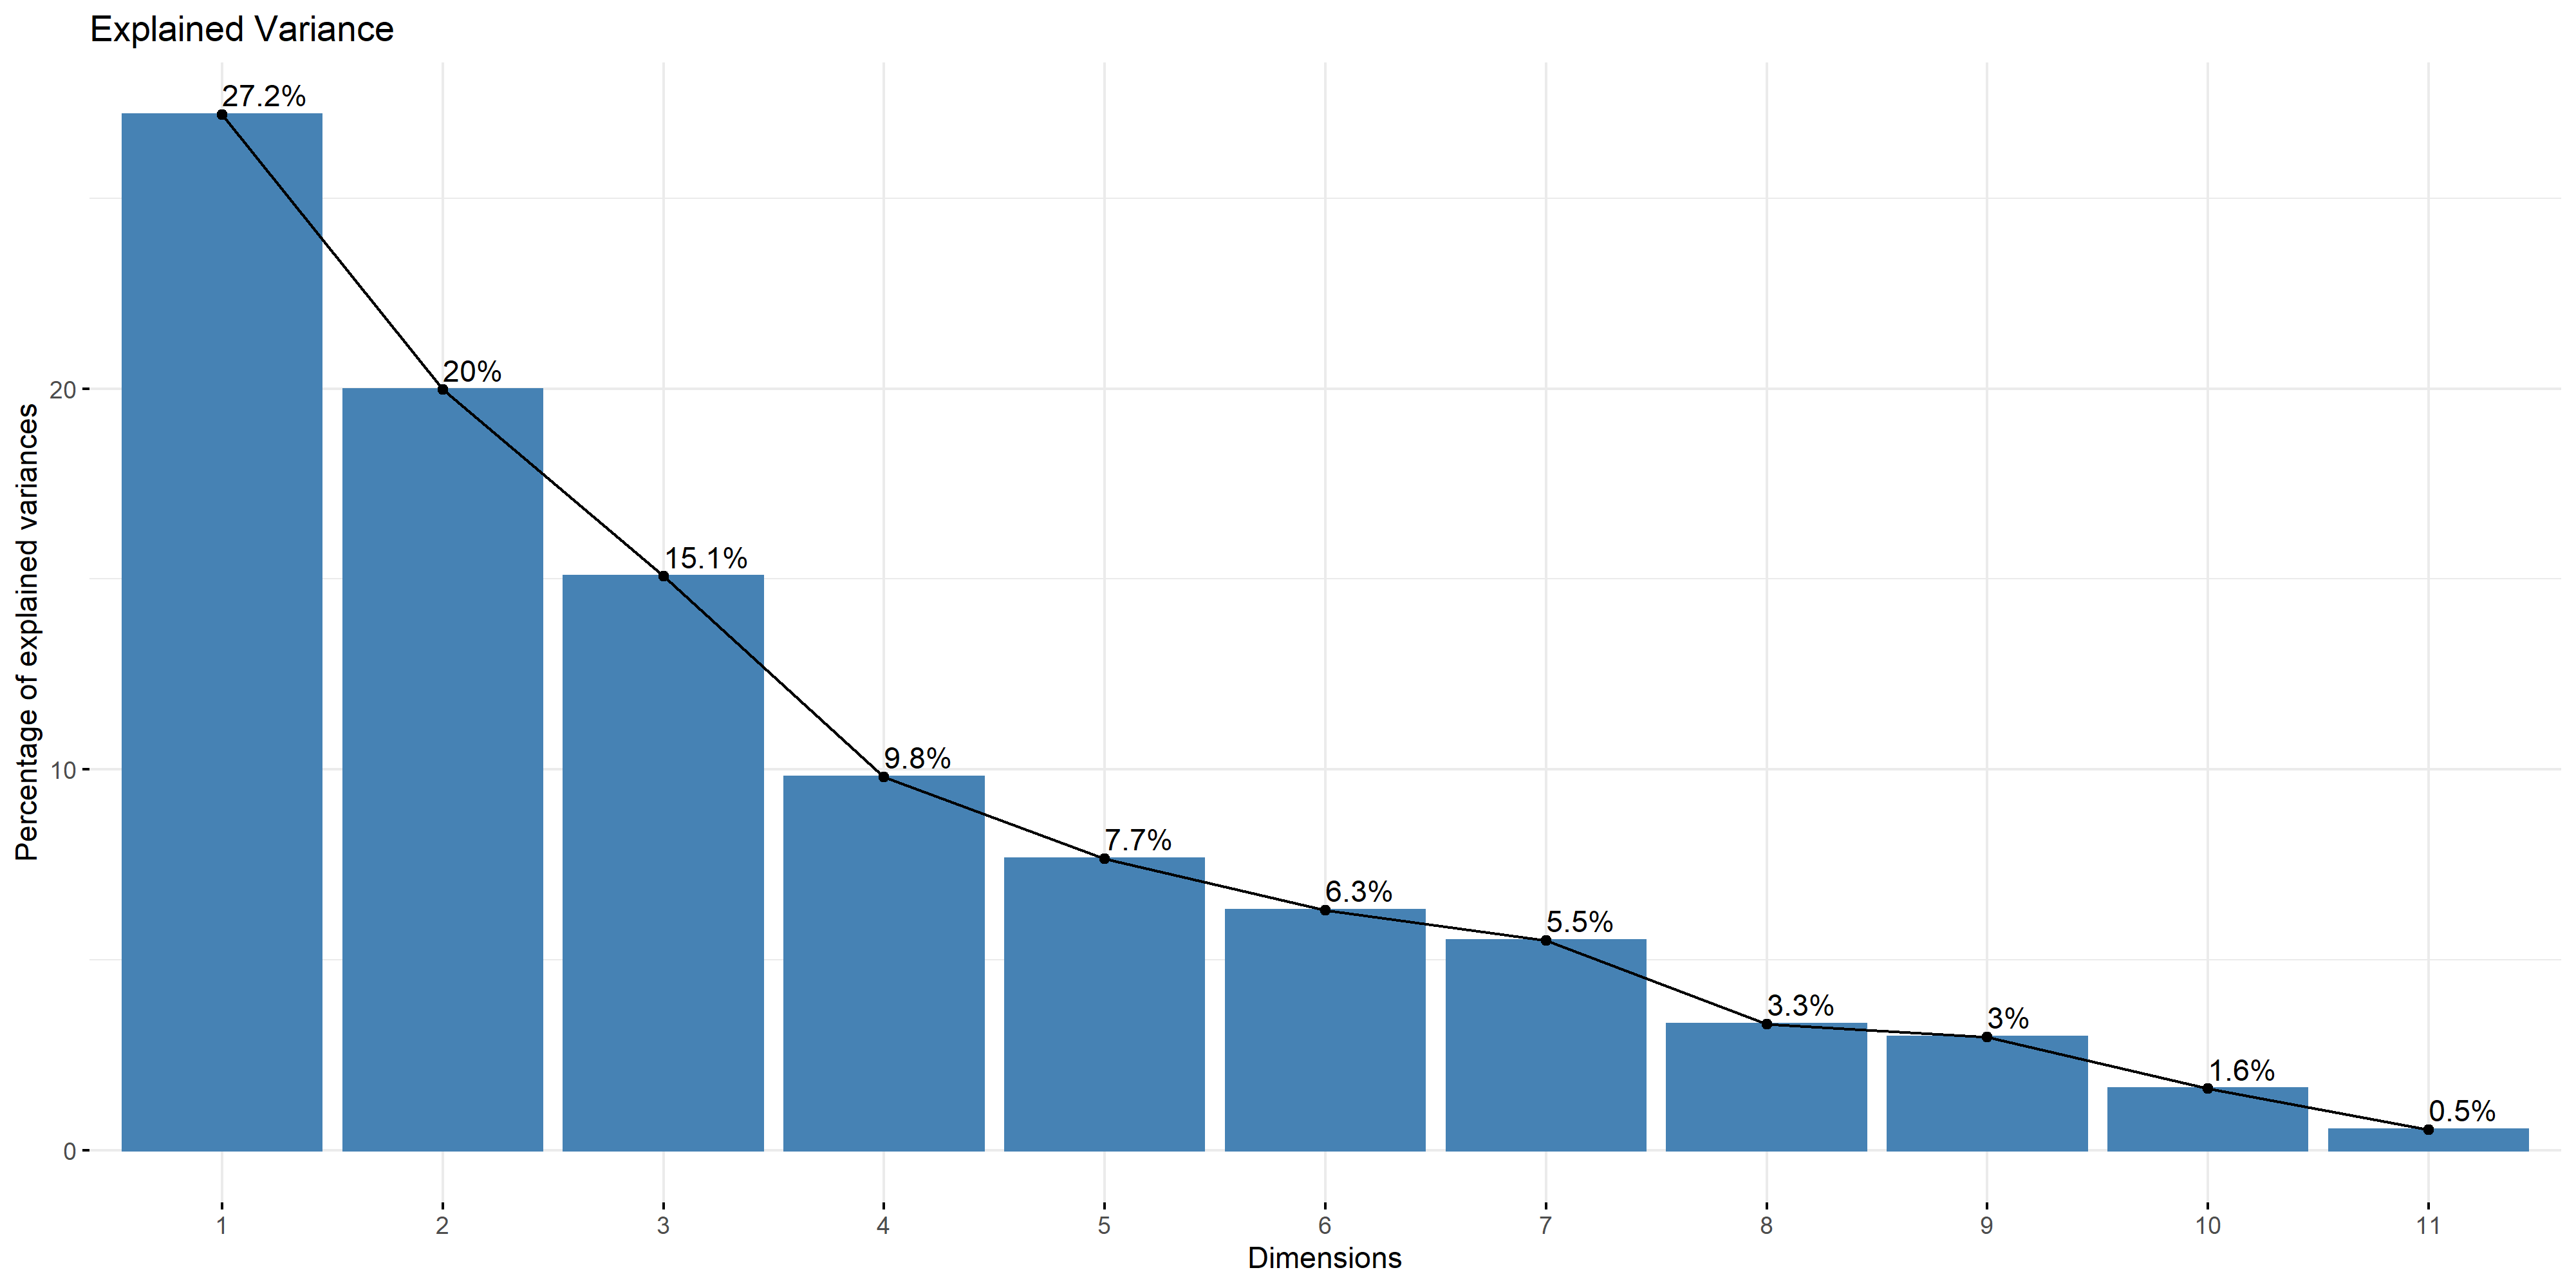
\includegraphics[scale=.4]{images/analisi/pca/variance_O.png}
    \caption{Questa immagine rappresenta la varianza spiegata per ogni componente della PCA.}
    \label{fig:variance_O}
\end{figure}

\begin{figure}[H]
    \centering
    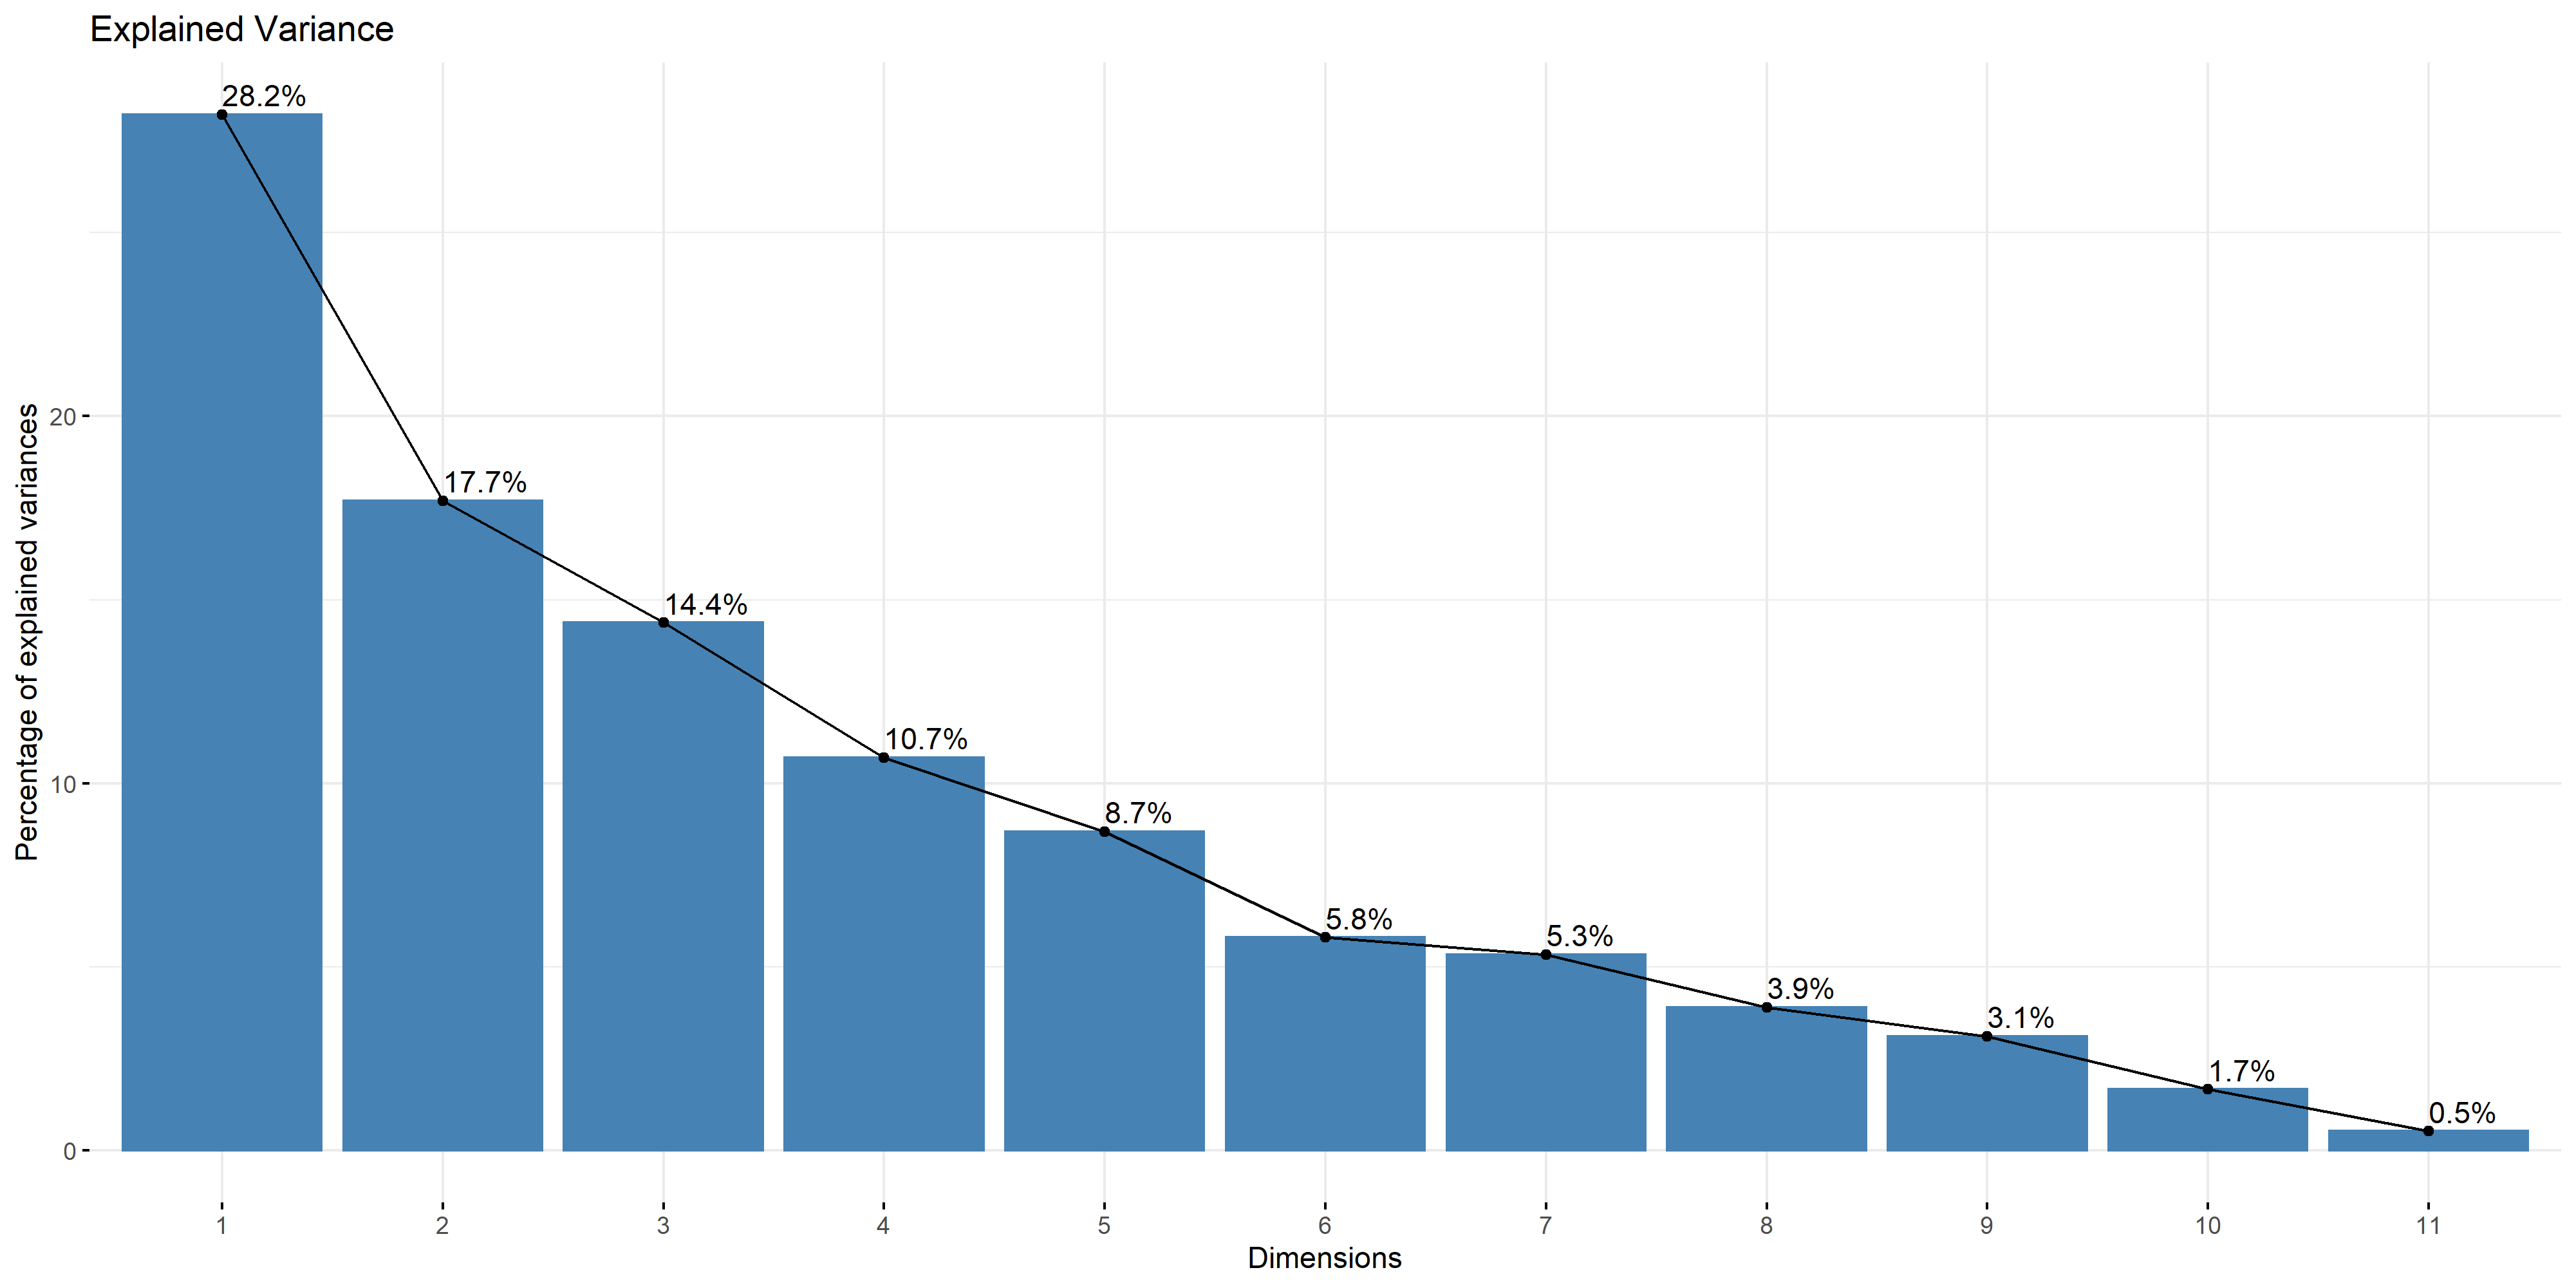
\includegraphics[scale=.4]{images/analisi/pca/variance_NoO.png}
    \caption{Questa immagine rappresenta la varianza spiegata per ogni componente della PCA; in questo caso dal dataset sono stati rimossi gli outliers.}
    \label{fig:variance_NoO}
\end{figure}
